% !TeX root = ../SDonchezThesis.tex

\chapter{Introduction}\label{ch:introduction}

Field Programmable Gate Arrays, or FPGAs, have long been utilized in devices benefiting from hardware acceleration of processes unsuitable for execution on a traditional processor, but which don't warrant the time consuming and cost-prohibitive process of ASIC design. FPGAs, in essence, enable a user to utilize a Hardware Development Language (HDL) to describe electrical circuits, which are then emulated using one of a number of techniques in a way that effectively mimics the actual physical construction of said circuits. However, unlike traditional physical circuits, FPGAs can be re-programmed as a user's needs change, resulting in tremendous improvements to iteration rates as well as development costs.

Traditional FPGAs, which consist solely of the programmable logic described above, have been widely replaced in industry with heterogenous systems, often comprising an FPGA alongside a ``Hard Processor System'' (HPS). In fact, modern designs such as Xilinx's Ultrascale+ MPSoC (Multi-Processor System on a Chip) line have tremendously complex architectures integrating multiple types of processors for varying applications, traditional programmable logic, dedicated digital signal processing, and more. A typical Ultrascale+ architecture is depicted in Figure \ref{fig:ultrascale}, below.

\begin{figure}
    \centering
    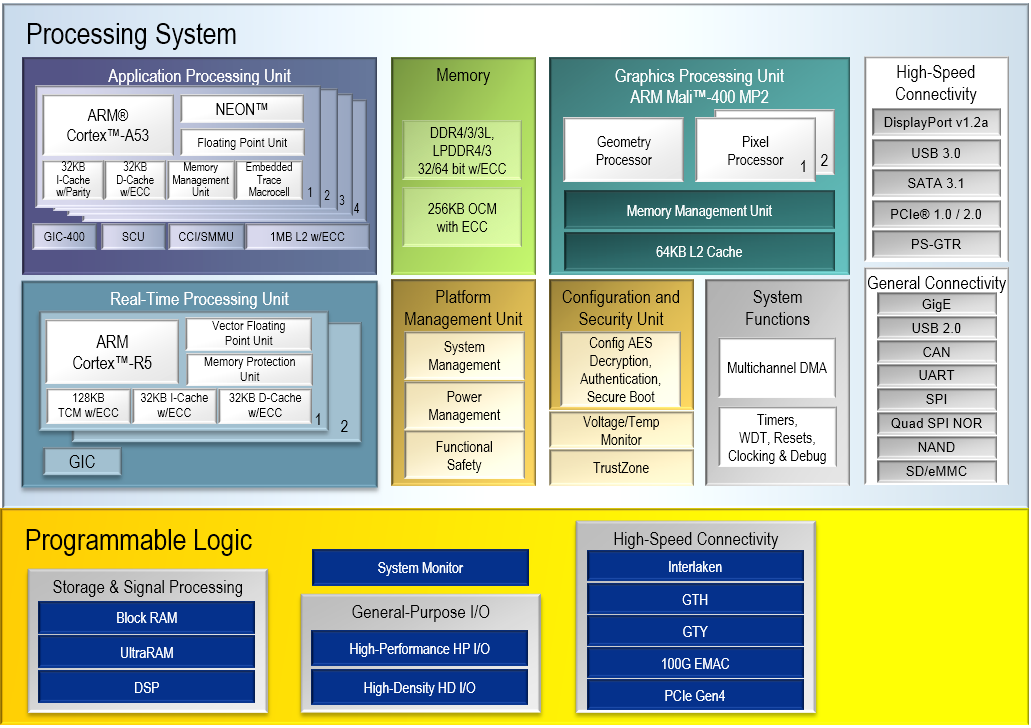
\includegraphics[width=0.8\textwidth]{zynq-eg-block.PNG}
    \caption[Typical Ultrascale+ Architecture]{Typical Ultrascale+ MPSoC Architecture \cite{noauthor_zynq_nodate}}
    \label{fig:ultrascale}
\end{figure}

Historically, such devices have been used extensively for prototyping, as well as in production devices, but generally in an environment where they are integrated into a dedicated device and intended for a single purpose. This closely parallels the history of much of traditional computing, wherein systems are geographically co-located with their users and associated with a single entity. 

However, the last decade has seen a massive shift in traditional computing away from on-premise compute resources in favor of third-party managed cloud computing. This transition has allowed increased flexibility and cost-efficiency for enterprise and personal users alike, and only continues to grow in ubiquity as time goes on. Accordingly, it should come as no surprise that, as much of the world pivots from on-site datacenters and computing resources to hybrid or cloud based platforms, Cloud Service Providers (CSPs) have shown an interest in providing FPGA-as-a-service resources to their tenants. Amazon, Alibaba, and Microsoft all offer such services as part of their respective cloud platforms, as do many of the other major players in the industry \cite{noauthor_amazon_nodate} \cite{noauthor_deep_nodate} \cite{noauthor_alveo_nodate}. 

Currently, these offerings mirror the traditional FPGA implementation - a single physical device per tenant instance. This is due to a variety of factors, mostly centered around device security for both the tenant and the CSP. However, research is underway that seeks to utilize Dynamic Partial Reconfiguration (DPR) as a means to enable CSPs to partition large FPGAs into multiple virtual devices, each of which can be allocated to a tenant. 

Dynamic Partial Reconfiguration is a process by which an FPGA can be partitioned into several reconfigurable regions (plus a static portion providing the reconfiguration functionality itself), each of which can be independently reloaded with a new design at any point in time. This enables tremendous flexibility for designers, especially in resource-constrained implementations. For example, an encryption/decryption platform can be dynamically reconfigured to enable the application of any of a number of algorithms, while needing an FPGA only a fraction of the size (and cost) of the one that would be needed to simultaneously host all of the various algorithms simultaneously. In the case of cloud applications, this enables each partition to be reprogrammed independently while others remain in service, enabling a single large FPGA to be partitioned for multiple end uses, or even end users.

This would allow CSPs to utilize much more economical devices, driving down cost for tenants and likely spurring increased adoption. However, the transition to partitioned multi-tenant devices is not trivial by any means. Before this technology can see widespread adoption, it must address a number of security concerns surrounding co-tenancy, as well as trust relationships between the CSP and the tenant.

This effort seeks to address these, that of the CSP - tenant trust relationship, alongside the hazards posed by co-tenancy, especially with a competitor or potential malicious actor. Understandably, many tenants are hesitant to provide their Intellectual Property (IP) directly to the CSP, as there is financial incentive for a CSP to integrate some of that IP into their own accelerator offerings. Furthermore, tenants may be limited by internal or governmental regulations with regards to the transmission of sensitive IP to other parties, including CSPs. 

Accordingly, tenants seek to upload encrypted IP to their partitions, with assurances that it is not possible for the CSP to directly access the decrypted content. This is feasible, and, even within the constraints of the multi-tenant scenario outlined above, has already been researched in academia. However, the solution posed in the literature is inefficient in its duplication of components, and furthermore contains a flaw that entirely violates the integrity of the bitstream as it pertains to its inaccessibility in its decrypted form by the CSP. This research effort seeks to address that vulnerability, while also providing performance enhancements to the original design. Specifically, this work, as a part of the larger effort, seeks to provide an efficient way of allocating shared decryption resources in a manner that reduces overhead while still ensuring the integrity of the IP's encryption through all CSP-accessible parts of the tenancy cycle.

\section{Motivation of this Research Effort}\label{Sec:motivation}
This research effort is primarily motivated by the obvious and immediate advantages that the implementation of multi-tenant FPGAs would bring to the industry. In addition to enabling CSPs to utilize more energy efficient and powerful devices, such a transition would likely drastically reduce the cost of such instances as they are offered to tenants, enabling more widespread adoption and unlocking the potential for tremendous growth, especially in the hot-topic and highly hardware dependent fields of Artificial Intelligence and Machine Learning.

This work is also motivated by the author's own interest in FPGA (and, more generally) SoC security, driven by experience both in academia and industry. The author hopes to provide a basis for further academic research in the future, as well as expand his own professional knowledge in the field.

\section{Research Goals}\label{Sec:goals}
This research effort seeks to enable the implementation of an efficient architecture for multi-tenant FPGA hardware in the cloud, thereby affording cost reductions to tenants and enabling greater adoption of the technology. Specifically this effort seeks to:

\begin{itemize}
    \item Enhance existing academic efforts to implement multi-tenant FPGA hardware in the cloud by reducing design overhead and increasing utilization of the resources required for multi-tenant use.
    \item Afford greater confidence in intellectual property and data security to tenants from malicious co-tenants by integrating robust memory isolation mechanisms into the proposed architecture.
    \item Transition the burden of trust away from the tenant-provider relationship onto the tenant-FPGA vendor relationship, as the latter has financial incentive to ensure the integrity of the tenant data with no potential ulterior motivations (which cannot be said about the provider).
\end{itemize}

\section{Organization of this Work}\label{sec:organization}
This work explores several individual facets of the architecture outlined above and expanded on in the subsequent chapters. Chapter \ref{ch:relatedWork} explores the state of academia with regards to the field of cloud-based multi-tenant FPGA devices, including a detailed analysis of the prior work which proposes the architecture this effort seeks to extend. Chapter \ref{ch:systemArchitecture} outlines the proposed enhancements to this architecture in detail, in preparation for the subsequent chapters which each discuss a particular aspect thereof.

Specifically, Chapter \ref{ch:edfScheduling} outlines the novel EDF scheduling algorithm proposed as a result of this research effort, which is utilized to allocate shared decryption resources between tenants equitably. Chapter \ref{ch:keyAggregateCryptography} explores the use of a key-aggregate cryptosystem to facilitate the easy encryption and subsequent decryption of the tenant bitstreams without requiring large key storage facilities to be implemented by the CSP. Meanwhile, Chapter \ref{ch:dmaProtection} explores the use of memory isolation functionality as made available in recent FPGAs, which greatly enhances the capacity of the CSP to provide meaningful isolation of data between tenants.  Chapter \ref{ch:conclusion} concludes this work, and provides a brief discussion of avenues for future research in this area.